%===================================
%===================================
%===================================
\setchapterpreamble[u]{\margintoc}
\chapter{SolarMED pilot plant}
\labch{solarmed:facility}

The \gls{solarmedLabel} system is an \gls{medLabel} plant that receives its
thermal energy from a solar field connected to a two-tank thermal storage
system. It is one of the experimental facilities located in \gls{psaLabel} as
can be seen in \reffig{intro:pilot-plants}.

The different components are interconnected as depicted in
\reffig{solarmed:facility:diagram}: a flat plate collector solar field which is
the heat source, a pressurized hot water two-tank thermal storage system, and
an \gls{medLabel} plant which uses this heat to separate seawater into fresh
water and brine. The solar field and thermal storage circuits are separated by
a heat exchanger. Two subsystems are differentiated: the \fullgls{sftsLabel}
subsystem and the thermal load that makes use of this heat for some useful
application, in this case, to produce separation by means of the
\gls{medLabel}: the separation subsystem.\todo{A esta figura quitar colores de
decision variable and environment variables, solo color neutro}

\begin{figure*}[h!]
	\includegraphics[]{figures/SolarMED-process-diagram.png}
	\caption{\gls{solarmedLabel} process diagram}
	\labfig{solarmed:facility:diagram}
\end{figure*}


\section{Heat generation and storage subsystem}
\labsec{solarmed:facility:sfts}

Two pressurized water tanks with a total capacity of 40 m$^3$ coupled to a
static solar field flat plate collectors with an aperture area of 606 m$^2$ and
a total thermal power of 323 kW$_{th}$ under nominal conditions.

\section{Separation subsystem}
\labsec{solarmed:facility:med}
The MED pilot plant was built in 1988
within the Solar Thermal Desalination project [REF]. It is a 14 effect,
vertically stacked, forward-feed plant initially built to use low-pressure
saturated steam as heat source for the first effect and later replaced to use
hot water within the XXX project in 2005. It has been operated in different
experimental campaigns and configurations robustly for more than two decades.
An image of the facility in its current state can be seen in
\reffig{solarmed:facility:med}. 


% Now the focus is to evaluate the potential gains by enabling and optimising the
% use of variable energy sources as well as its application for brine
% concentration. 
Some particularities of this system are explained hereinafter:

\begin{itemize}
    \item VFDs are used to control all flow rates in the system: heat source, cooling, feed, brine and distillate.
    
    \item As mentioned, the external heat source driving the process, is hot water from a thermal storage system. Water is drawn from one of the tanks and mixed with the water at the outlet of the first effect through a three-way valve, allowing independent regulation of flow and temperature.
    
    \item The inland location of this experimental plant is another particularity of the system. A fixed amount of seawater (30 m$^3$), stored in a reservoir, is available to be used in the process and replenished as needed. The effluents from the plant are mixed in a different reservoir (5 m$^3$), and returned to the feed in a close loop operation. Because water exits the process at a higher temperature than when it enters, this type of operation implies an ever-increasing heat sink temperature. A wet cooling tower, installed between the two reservoirs, is used to mitigate this effect.

    \item The previous particularity leads to a significant variation in the inlet water temperature from day to day and also within the same day depending on the operation conditions. To ensure the stability of the condenser (i.e. a constant vapor pressure and outlet cooling water temperature), the cooling flow rate is regulated. This allows to have a stable system representative of a real plant operating under normal conditions. However, this can lead to variable electrical consumption of the cooling pump.

    \item The vacuum system of the plant is based on two hydro-ejectors and a pump. The pump is operated always at fixed speed and its electrical consumption has been characterized with measurements under various conditions as being near-constant and independent of the operation conditions. Its associated nominal power is 5 kW$_e$.

    \item The salinity of the feedwater is checked before every test measuring its conductivity with a conductivity meter (see Table \ref{tab:results_instrumentation}).

    % \item The distillate conductivity is measured every few tests in order to validate the proper operation of the plant (demisters, leakages, etc). The measurement of this variable is not considered necessary for each operating point, since a small variation in the order of 0.05 to 0.3 g/kg has been observed and therefore not deemed to have a significant effect on the results.
    % \item Brine and distillate extraction are controlled by keeping its respective levels constant by means of feed frequency regulation of the respective pumps. 
\end{itemize}

\begin{marginfigure}[-8cm]
	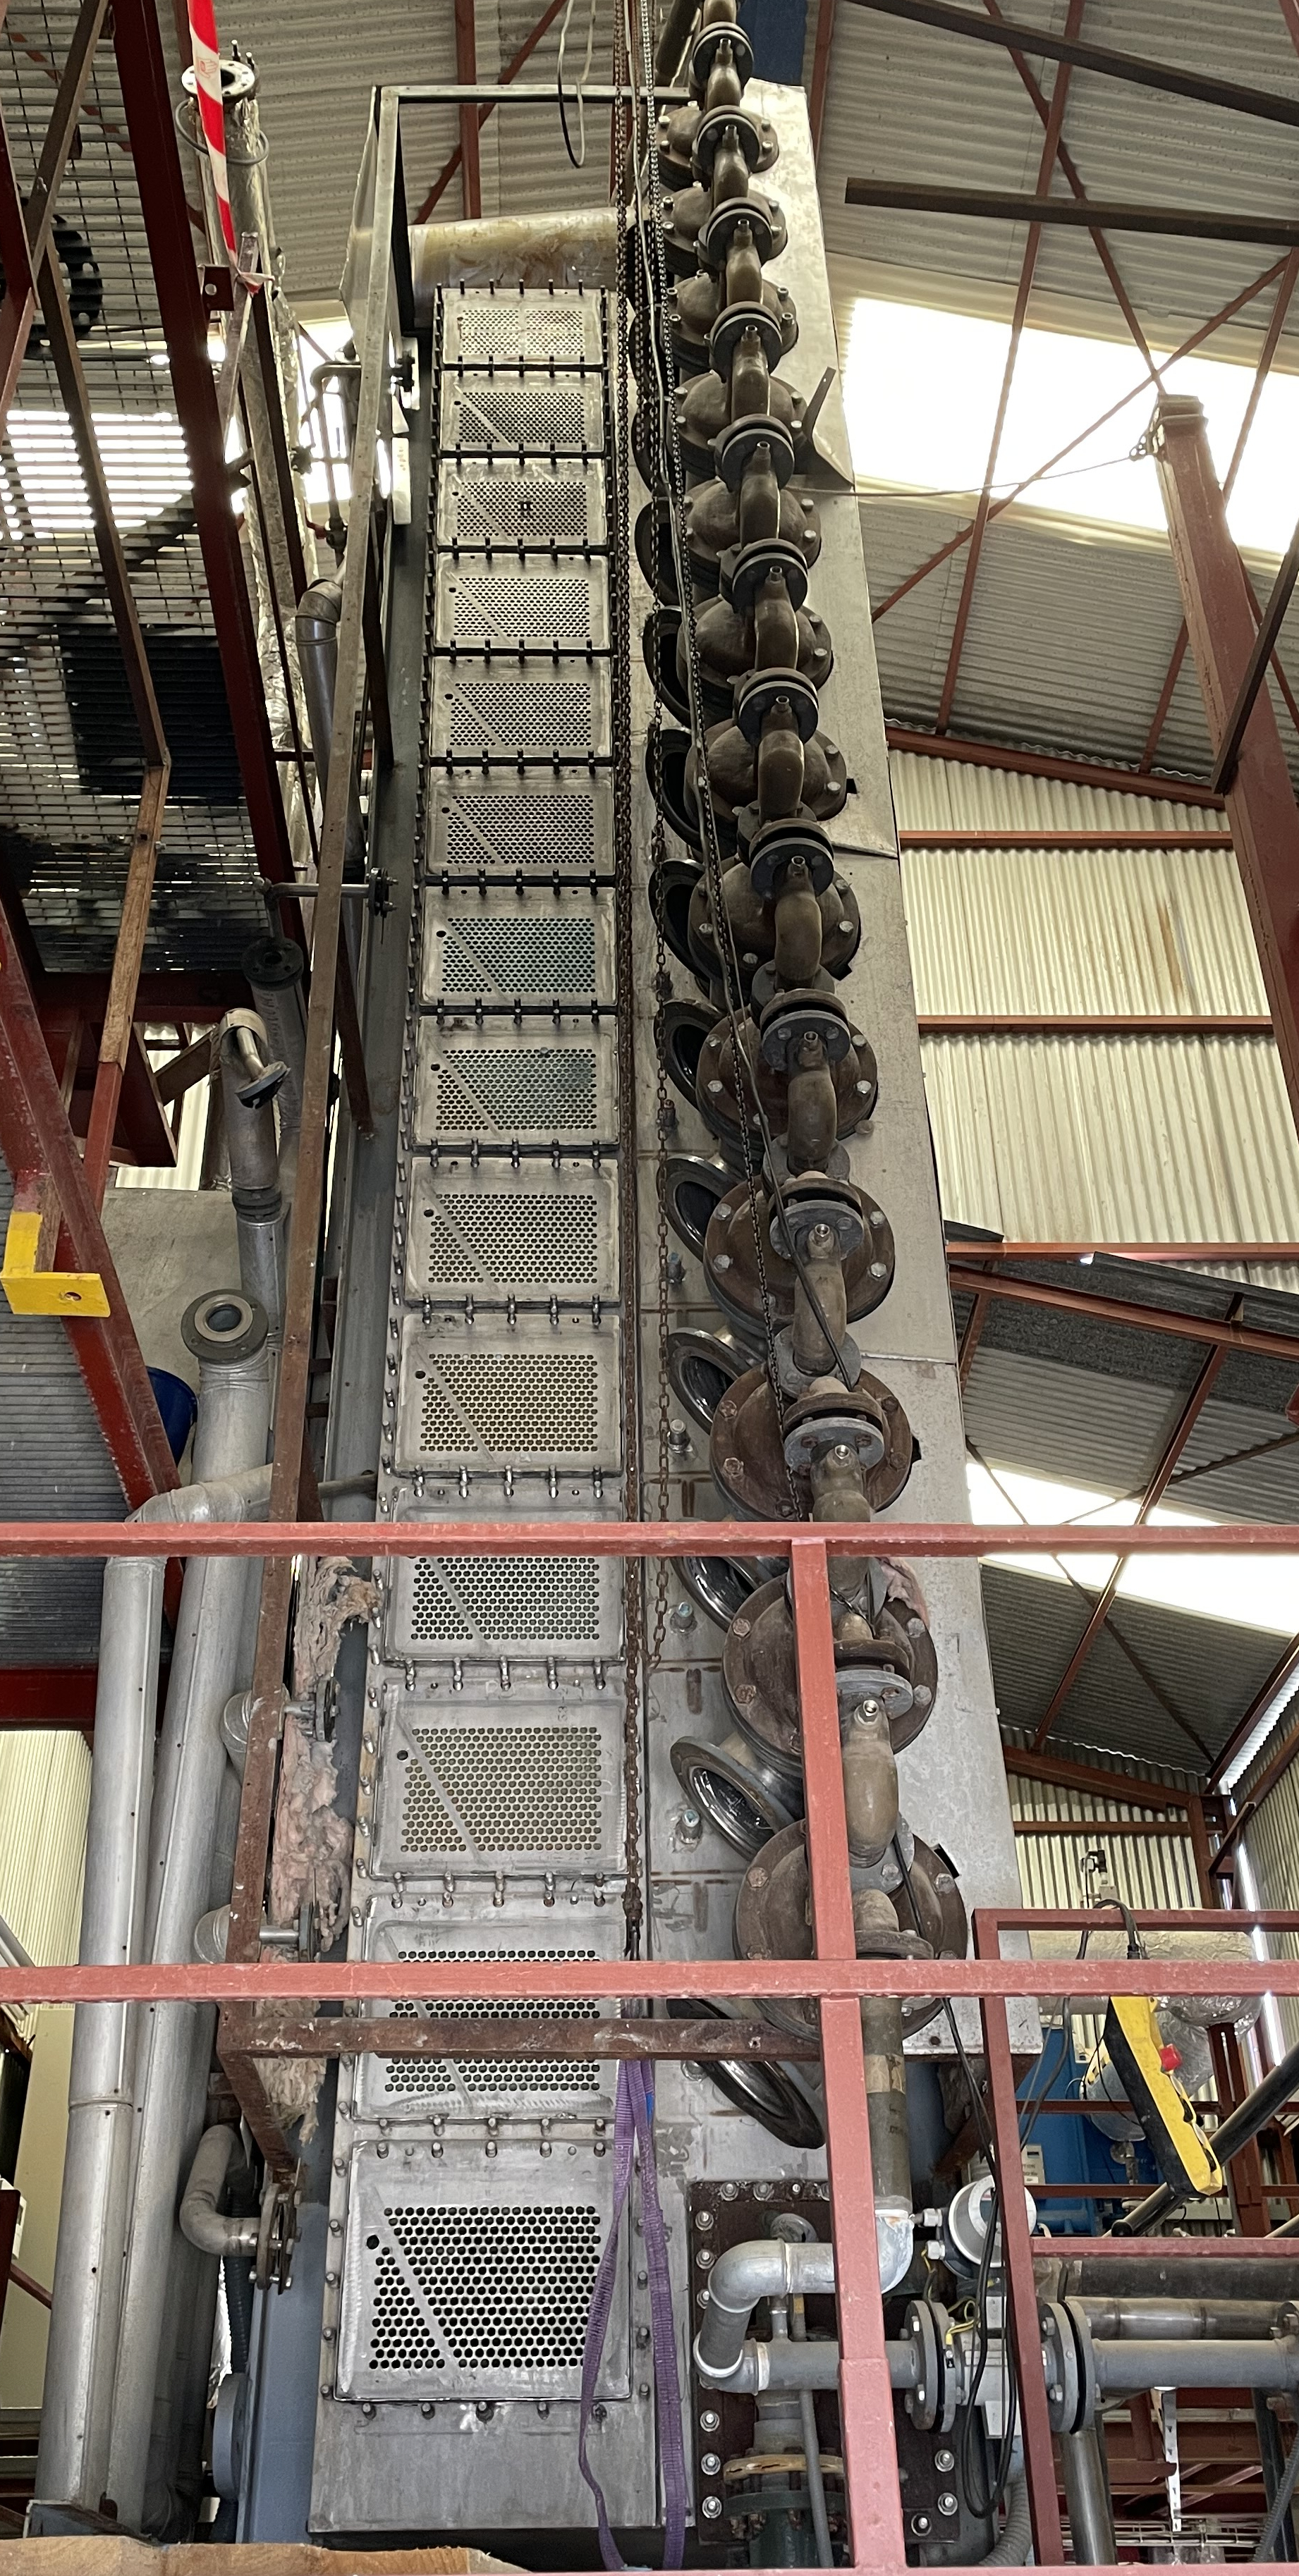
\includegraphics[width=.8\textwidth]{figures/solarmed-facility-med.jpg}
	\caption{\gls{medLabel} plant at \gls{psaLabel} with open effects for maintenance}
	\labfig{solarmed:facility:med}
\end{marginfigure}

A summary of its main specifications is shown at Table
\reftab{solarmed:facility:specifications}.

\begin{margintable}[]
    \caption{\gls{medLabel} plant at \gls{psaLabel} specifications and nominal operating conditions}
    \labtab{solarmed:facility:specifications}
    \resizebox{\linewidth}{!}{%
	\begin{tabular}{@{}rl@{}}
	\toprule
	\multicolumn{1}{r}{\textbf{Parameter}} & \multicolumn{1}{l}{\textbf{Value}} \\ \midrule
	Capacity                               & 72 m³/day                          \\
	Number of effects                      & 14                                 \\
	Feed type                              & Forward feed                       \\
	Physical arrangement                   & Vertically stacked                 \\
	Heat exchanger configuration           & 90/10 Cu-Ni HTE                    \\
	Heat source type                       & Hot water                          \\
	Vacuum system                          & Hydro-ejectors                     \\ \midrule
	Heat source flow rate                  & 12 L/s                             \\
	Feed water flow rate                   & 8 m³/h                             \\
	Brine rejection                        & 5 m³/h                             \\
	Distillate production                  & 3 m³/h                             \\
	Cooling flow rate at condenser         & 8-20 m³/h (10-25 $^{\circ}$C)               \\
	Thermal power consumption              & 190 kW                             \\
	Top Brine Temperature (TBT)            & 70 $^{\circ}$C                              \\
	Condenser temperature                  & 35 $^{\circ}$C                              \\ \midrule
	\multicolumn{1}{l}{}                   &                                    \\
	\multicolumn{1}{l}{}                   &                                    \\
	\multicolumn{1}{l}{}                   &                                    \\
	\multicolumn{1}{l}{}                   &                                   
	\end{tabular}
	}
\end{margintable}


The facility's instrumentation is shown in
\reftab{solarmed:facility:instrumentation}. As can be seen, \gls{pt100Label}
sensors are used to measure all liquid temperatures
(\texttt{TT01}..\texttt{TT05}), while a PT1000 sensor is used to
measure the ambient temperature (\texttt{TT06}). The pressure inside the first
effect and condenser (\texttt{PT01} and \texttt{PT02}, respectively) is
measured by two different pressure transducers which fundamentally differ in
their measurement range. To monitor the power consumption of the system,
various subsystems have been individually instrumented using a power meter
(\texttt{JT01}..\texttt{JT04}). Conductivity is measured using a portable
conductivity meter (\texttt{CT01}, \texttt{CT02}), to which a calibration is
periodically performed to convert conductivity to salinity. Flow rates
(\texttt{FT01}..\texttt{FT04}) are measured using different types of flowmeters
depending on the characteristics of the fluid being evaluated. Electromagnetic
flowmeters are used for conductive fluids, while vortex flowmeters are used for
non-conductive fluids. All sensors transmit a \mbox{4--20 mA} analog signal
that is converted to digital by \gls{adcLabel} converters.

\begin{table}[]
\caption{Characteristics of the instrumentation installed at MED-PSA unit ($^a$ value of the measured temperature in $^\circ$C, $^b$ of reading, $^c$ full scale).}
\labtab{solarmed:facility:instrumentation}
\resizebox{\textwidth}{!}{%
    \begin{tabular}{@{}ccccc@{}}
    \toprule
    \textbf{Measured variable} & \textbf{Instrument} & \textbf{Model} & \textbf{Range} & \textbf{Measurement uncertainty} \\ \midrule
    Water temperature, TT01...TT0N & PT100 Class A & SEDEM OF112871 & 0 - 100$^\circ$C & $\pm$ 0.15 + 0.002$\cdot T^{a}$ \\
    Distillate flow rate, FT03 & Vortex flow meter & ABB TRIO-WIRL VT4 & 1.6 - 18 m$^3$/h & $\pm$ 0.75\% o.r.$^{b}$ \\
    Hot water flow rate, FT01 & Electromagnetic & \begin{tabular}[c]{@{}c@{}}Endress+Hauser \\ Proline Promag 50P\end{tabular} & 2.42 - 78.33 L/s & $\pm$ 0.5\% o.r. \\
    Feedwater flow rate, FT02 & Electromagnetic & \begin{tabular}[c]{@{}c@{}}Endress+Hauser \\ Proline Promag P 300\end{tabular} & 2.1 - 66 m$^3$/h & $\pm$ 0.5\% o.r. \\
    Ambient temperature, TT05 & PT1000 & - & -40 - 60 $^\circ$C & $\pm$ 0.15 + 0.002$\cdot T$ \\
    Pressure, PT01 & Pressure capacitive & \begin{tabular}[c]{@{}c@{}}Endress+Hauser\\ Cerabar T-PMC131\end{tabular} & 0 - 1 bar & $\pm$ 0.5\% FS$^{c}$ \\
    Pressure, PT02 & Piezoresistive sensor & WIKA S-10 & 0 - 0.6 bar & $\pm$ 0.5\% FS \\
    Level, LT01, LT02 & Magnetic level gauge & IGEMA NA7-50 & 0-750 mm & $\pm$ 5 mm \\
    Power, JT01...JT04 & \begin{tabular}[c]{@{}c@{}}Power meter Class 1\\ IEC 62053-21\end{tabular} & Circutor CM31 & 0-7 kW & $\pm$1\% o.r. \\
    Conductivity, CT01...CT02 & Conductivity meter & \begin{tabular}[c]{@{}c@{}}Prominent \\ Portamess 911\end{tabular} & 0.1$\mu$S/cm - 1000 mS/cm & \begin{tabular}[c]{@{}c@{}}$\pm$ 0.5\% o.r. < 500 mS/cm\\ $\pm$ 1\% o.r. $\geq$ 500 mS/cm\end{tabular} \\ \bottomrule
    \end{tabular}%
}
\end{table}